\section{In-lab Experiments}
\label{sec:inlab}

%%%%%%%%%%%%%%%%%%%%%%%%%%%%%%%%%%%%%%%%%%%%%%%%%%%%%%%%%%%%%%%%%%%%%%%%%%%%%%%%

We start our evaluations of {\myit} using controlled in-lab experiments to  analyze and understand the performance of {\myit} under  different experimental settings. Specifically, we measure the power usage for different culling angles, 
focal angles, and motion dynamics to capture the impact of each {\myit} feature,
(1) culling, (2) mesh simplification, and (3) screen dynamics-based frame rate 
control, respectively. We also gathered qualitative measurements using a small-scale user study of five participants to understand how parameter changes in the three  criteria affects the perceived object quality to determine the appropriate values for our application-oriented user studies (discussed in Section~\ref{sec:userstudies}). 


%%%%%%%%%%%%%%%%%%%%%%%%%%%%%%%%%%%%%%%%%%%%%%%%%%%%%%%%%%%%%%%%%%%%%%%%%%%%%%%%

\subsection{Culling Angle}

\begin{figure}[t]
    \centering
    \vspace{-1ex}
    \subfigure[Total power usage]{
       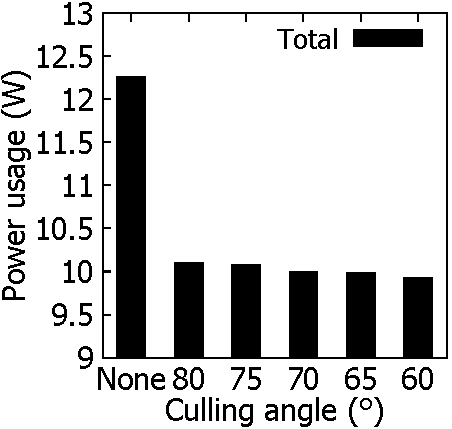
\includegraphics[width=0.45\linewidth]{Culling_cropped}
        \label{fig:lpgl-cullingangle}
    }
    \subfigure[GPU/memory power usage]{
        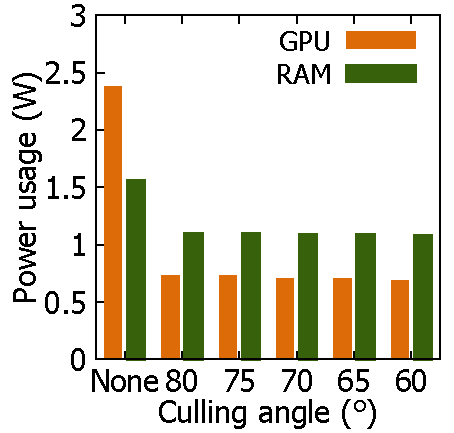
\includegraphics[width=0.45\linewidth]{Culling_GPU_RAM_cropped}
        \label{fig:lpgl-cullingangle-gpu}
    }
    \vspace{-2ex}
    \caption{Power consumption for enabling
            {\myit}'s culling at different angles.}
    \label{fig:lpgl-cullingangle-all}
\end{figure}


To identify the optimal culling angle for the {\mlo}, we first built an application to display 72 small bunnies horizontally with the center bunny (right in front of the user's field of view) colored in green and the other 71 colored in white, arranged evenly in a 360$^\circ$ circle around the participant -- with each bunny separated by its neighbor by $360/72=5^\circ$. During the experiment, we asked each participant to focus their attention on the green bunny and inform us when they noticed something changing in the scene. We then slowly removed bunnies from the scene starting with the leftmost and rightmost bunnies (they were always removed in matching pairs) until the participant noticed something changing in their visible scene.

This experiment was designed to identify the visual angle at which participants could notice changes to the scene with their peripheral vision. This angle is important to know as objects outside this noticeable area can be culled by {\myit} (i.e. not rendered) to save power. On the {\mlo}, the effective maximum field of view is 80$^\circ$ -- thus we started our tests from 80$^\circ$, as anything larger would not be visible anyway (as the {\mlo} would not display it).

Figure~\ref{fig:lpgl-cullingangle-all} shows the reduction in power consumption as the culling angle moves from ``None'' to 80$^\circ$ and lower. We observe that, depending on the scene complexity, significant amounts of power (20\% or more) can be saved by not rendering objects that cannot be seen by the user. However, this culling has to be balanced with usability. From our study, we noticed that, due to the small field of view of the {\mlo}, any culling in the visible area was immediately noticed by the participants. Thus, despite increased power savings potential, to maintain the user experience, we set the culling angle for the {\mlo} to 80$^\circ$ (to match its small field of view) in all future experiments.


%We designed a static application is spreading many white little bunnies in front side and middle green bunnies to focus the middle side. Under such conditions, we target to observe the performance of {\myit}'s culling algorithm as it analyzes the angle of the current scene. Specifically, we use tiny bunnies. When changing culling angles, we want to check fine angles for finding a suitable parameter. The focus angle's level 1 is 10$^\circ$ and level 2 is 60$^\circ$ is based on our preliminary quality studies. From the bars in \fig\ref{fig:lpgl-cullingangle} we can see that even at 80$^\circ$ (performance-wise worst case for {\myit}), when applying {\myit}, the energy consumption is lower compared to the baseline. 


%%%%%%%%%%%%%%%%%%%%%%%%%%%%%%%%%%%%%%%%%%%%%%%%%%%%%%%%%%%%%%%%%%%%%%%%%%%%%%%%

\subsection{Focal Angle}


\begin{figure}[t]
    \centering
    \vspace{-1ex}
    \subfigure[Total power usage and 5-point Likert-scale score on scene quality]{
       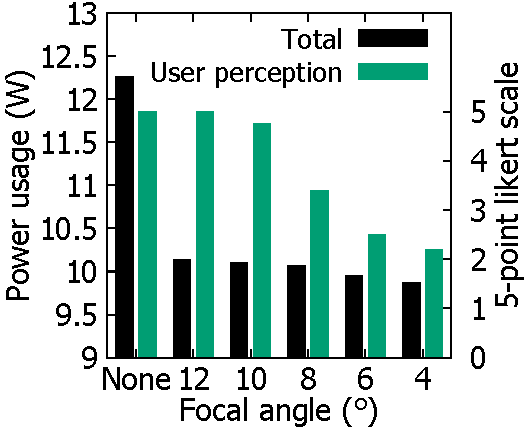
\includegraphics[width=0.49\linewidth]{Focus_cropped}
        \label{fig:lpgl-focusangle}
    }
    \subfigure[GPU/memory usage]{
        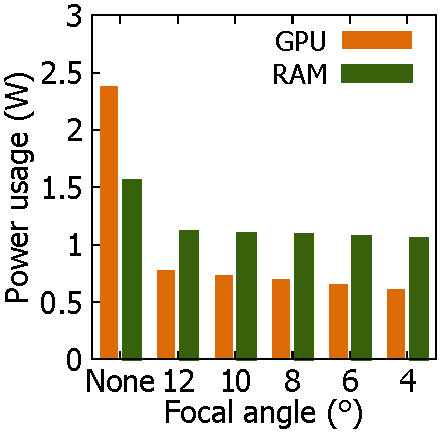
\includegraphics[width=0.409\linewidth]{Focus_GPU_RAM_cropped}
        \label{fig:lpgl-focusangle-gpu}
    }
    \vspace{-2ex}
    \caption{Power consumption and scene quality perception scores for
            varying core focal angles.}
    \label{fig:lpgl-focusangle-all}
\end{figure}

{\myit} defines two types of focal angles: \textit{peripheral focal angle} and \textit{core focal angle}. For objects that are farther away
than the peripheral focal angle, a very simple mesh is presented 
(level 2 simplification), and for objects within the \textit{core focal angle} 
the highest quality mesh is presented. If the object is located between these two angles, a level 1 simplified mesh is displayed. We set the peripheral focal angle to 60$^\circ$ based on findings from previous literature~\cite{Grosvenor07, Bhise11}, and used the culling angle application to understand the impact of changing the core focal angle on the power and user perception, except for this experiment, we placed the bunnies $2^\circ$ apart to observe any effects at  finer granularity.


During the study, we randomly set the core focal angle to different values and asked the participants to focus on the green bunny in the center and rank the quality of the scene using a 5-point Likert scale (very low: 1, very good: 5). With decreasing core focal angles, the bunnies that are located close to the user-focused green bunny will start to be presented as a simplified mesh. Our results, shown in \fig\ref{fig:lpgl-focusangle-all} for both power consumption and user perceived quality, suggest that the participants started to quickly notice changes when the core focal angle was smaller than 10$^\circ$. Again, similar to the culling angle, despite the power benefits of a narrow core focal angle, we set the focal angle to 10$^\circ$ to minimize the usability impact.


%
%However, based on the findings from the previous experiment, we fixed the 
%culling angle at 80$^\circ$.
%(the angle distance from the user's focal point up to where the high quality objects are drawn) 
%

%
%


%From our user study, we noticed that having a core focal angle higher than
%10$^\circ$ did not show any differences on the user perception levels.
%In \fig\ref{fig:lpgl-focusangle} we present the energy consumption for the 
%{\mlo} for different core focal angle values. If an object resides within the
%core focal angle, a high quality representation of the 3D object is presented 
%on the screen. Therefore, as we decrease the angle, we see lower energy usage 
%at a device-scale, mostly due to the reduction of energy usage at the GPU and
%memory. Nevertheless, given that the goal of {\myit} is to maintain the user 
%perception while reducing energy consumption, we keep the core focal range to
%10$^\circ$ in the following experiments.


%We start changing level 1 focal angle at 12 based on our preliminary studies. Because people don't noticed that something is strange when focal angle is over 12. We can see that \fig\ref{fig:lpgl-focusangle}, increasing level 1 focal angle, energy usage is increased.


%%%%%%%%%%%%%%%%%%%%%%%%%%%%%%%%%%%%%%%%%%%%%%%%%%%%%%%%%%%%%%%%%%%%%%%%%%%%%%%%

\subsection{Object Speed and Frame Rate}


\begin{figure}[t]
    \centering
    \vspace{-1ex}
    \subfigure[Total power usage and achieved frame rate for varying object speeds]{
       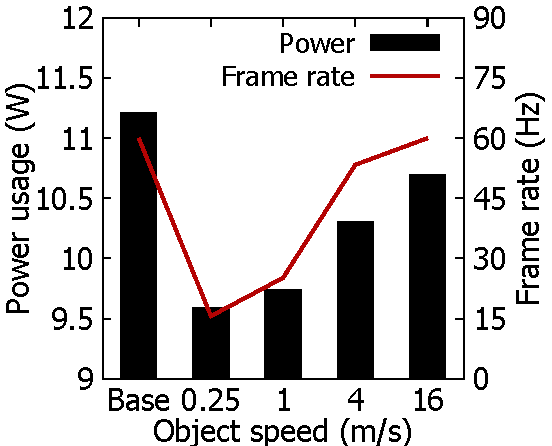
\includegraphics[width=0.49\linewidth]{objectSpeed_cropped}
        \label{fig:lpgl-objSpeed}
    }
    \subfigure[GPU/memory usage]{
        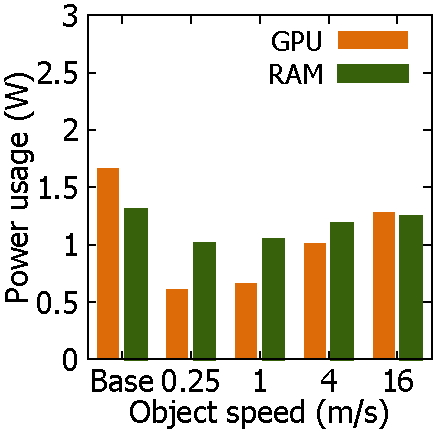
\includegraphics[width=0.409\linewidth]{objectSpeed_GPU_RAM_cropped}
        \label{fig:lpgl-objSpeed-gpu}
    }
    \vspace{-2ex}
    \caption{Power consumption and scene quality perception score for varying object speeds.}
    % which impact {\myit}'s frame rate control.}
    \label{fig:lpgl-objSpeed-all}
\end{figure}


Next, to investigate the impact of {\myit}'s dynamic frame rate control, we conducted an experiment where four 69K triangle bunnies are moved up and down the scene.  We varied the speed of the bunnies from 0.25-16~m/s keeping each bunny 5 meters away from the user. At 0.25~m/s (low dynamics), we expect {\myit} to use a low frame rate (15 fps), while at 16~m/s, we expect {\myit} 
to use the maximum frame rate (60 fps). {\myit} uses three levels of frame rates, 15, 30 and 60 fps, and we configured it, based on our initial user tests, to move from 15 to 30 fps if, across two frames, at least one object moves across more than 15\% of the entire scene. If an object moves across more than 30\% over two subsequent frames, we set the frame rate to 60 fps.
%
From the results, shown in \fig\ref{fig:lpgl-objSpeed-all}, we note that even at 60 fps displaying the same objects, {\myit}'s power consumption is lower 
compared to the baseline (due to culling, focal angle etc.) and that it's consumption rate is much lower at lower fps.

%

%Notice in the line plot of \fig\ref{fig:lpgl-objSpeed} that with increasing %object speeds, {\myit} increases its frame rate gradually from 15 to 60 fps.
%When not using {\myit} (baseline rendering of {\mlo}), the frame rate is always %fixed to its default 60 fps.
%
%
%Furthermore, my comparing \figs\ref{fig:frame_rate} %and~\ref{fig:lpgl-objSpeed-all},
%despite having the same number of draw calls (i.e., four), object complexity, and %frame rate, applying {\myit} shows lower energy consumption rates.
%
%Such reductions are mostly from the lowered power usage of the GPU and memory %(\fig\ref{fig:lpgl-objSpeed-gpu}). Our observations can be explained by the fact %that {\myit}
%tries to not only actively lower the frame rate with respect to the screen
%dynamics, but it comprehensively applies other features such as culling and 
%mesh simplification to minimize the devices' energy consumption rate as a whole. 


%%%%%%%%%%%%%%%%%%%%%%%%%%%%%%%%%%%%%%%%%%%%%%%%%%%%%%%%%%%%%%%%%%%%%%%%%%%%%%%%

%\subsection{Object quality for focused regions}

%\begin{figure}[t]
%    \centering
%    \vspace{-2ex}
%    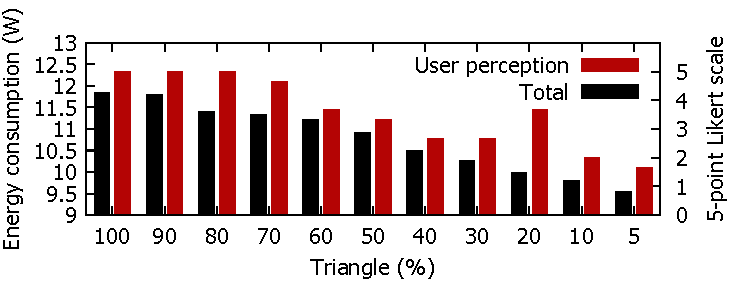
\includegraphics[width=0.8\linewidth]{objectQuality_cropped}
%    \vspace{-2ex}
%    \caption{Power consumption and perception scores for varying object qualities (triangle %usage percentages with respect to original 69K triangle object).}
%    \label{fig:lpgl-optimized}
%\end{figure}

%Next, we validated the effort of different object quality levels on both power consumption and user perception by presenting to our test users 11 different Stanford bunnies -- each  with different triangle counts. \fig\ref{fig:lpgl-optimized} presents the power consumption for each case along with the user perceived quality scores on a 5-point Likert scale. We observed that the power consumption decreased linearly while the user perception was high until after the 70\% mark.  

%Furthermore, given the power consumption reduction-to-usability trade off in %\fig\ref{fig:lpgl-optimized} and qualitative feedback from the study participants %(indicating that quality loss beyond the focal angle was not disturbing), we %select level 1 simplified objects to contain 10\%, and level 2 simplified objects %to contain 5\% of the original triangle 


%This suggests that even if we were to use a reduced triangle object of 70\% of %the original (even for objects in the core focal angle), the users would not know %a significant difference in usability.
%%
%
%we presented nine different 3D objects of varying
%triangle count (object size 1~m in height at 2~m distance) to nine users.
%
%Specifically, the Stanford Bunny that we present has the original number of
%triangles in the 100\% case, but this triangle count decreases by 10-90\%. 
%
%count. 


%
%These results suggest that spending energy to render objects at higher fidelity
%than 70\% of the original will not have a significant impact on the 
%system's usability aspect.
%
%In other words, even if the user is gazing at a specific object (i.e., object 
%is within the core focal angle), we can present a simplified object to conserve
%energy. 
%
%Therefore, we can further optimize the performance of {\myit} using such 
%quality thresholds; 

%\jk{I don't like this statment... but that's what we have...}

%Note that in this experiment we made a small change to the Stanford Bunny so that the bunny had a sphere plugged in to its left eye as in \fig\ref{fig:user-bunny}(c). Four of our five study participants noted that the sphere started to look different 


%%%%%%%%%%%%%%%%%%%%%%%%%%%%%%%%%%%%%%%%%%%%%%%%%%%%%%%%%%%%%%%%%%%%%%%%%%%%%%%%

\subsection{Latency Overhead}

%\begin{figure}[t]
%    \centering
%    \vspace{-2ex}
%    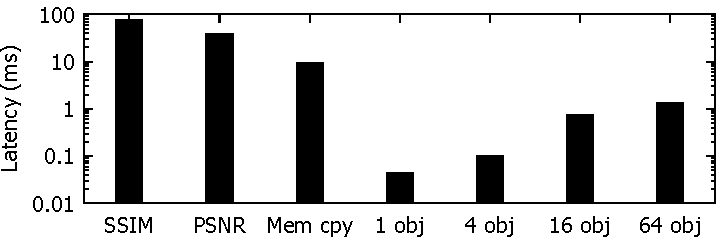
\includegraphics[width=0.8\linewidth]{latency_cropped}
%    \vspace{-2ex}
%    \caption{SSIM, PSNR, and {\myit} Latency}
%    \label{fig:latency}
%\end{figure}

We now analyze the latency of {\myit}, in particular the latency it adds to the rendering pipeline.  We found that the additional latency per-object for {\myit} was 45.57$\mu$sec. As the number of objects increases, the overall latency of {\myit} increases sub-linearly and was $\sim$1.2ms for 32 objects and $\sim$2.5ms for 64 objects. In addition, the latency to perform {\myit}'s run-time object simplification for dynamical loaded objects is 819~msec when simplifying a 69K triangle object to 50\%. This long latency is fortunately a one time process when the object is first used. Later when the object is re-used, {\myit} loads the pre-simplified object to the scene with minimal latency. Overall, the latency of {\myit} is low and does not add any noticeable delay.

%\fig\ref{fig:latency} show the {\myit} latency when  
%1 to 32 objects are presented on the scene. 
%, the overall added latency was still less than 1 ms (as the 
%we see increasing latency, but still noticeably lower than 
%the latency introduced by PSNR and SSIM by multiple orders of magnitude. 


%, and also compare with other frame
%similarity metrics widely used for frame dynamics computation 
%(e.g., SSIM and PSNR).
%
%Note that both SSIM and PSNR are computed for the entire frame as a whole;
%therefore, it does not scale with the number of objects. 
%However, they add the overhead of copying GPU frame buffer contents to the 
%memory for frame dynamics computation. 
%

%
%Specifically, the latency introduced when determining the mesh simplification
%level and culling range is static for any scene, given that these decisions 
%are made based on the mobile device's field of view and the predefined parameters 
%mentioned above. On the other hand, 
%
%This latency will be affected by the number of objects that are displayed
%given that {\myit} operations are dependent on the bounding-box of \textit{each} %object. 
%With more objects, {\myit}'s RDCC would iterate more. 
%

%\fig\ref{fig:latency} and also compare its performance with other frame similarity metrics that are widely used for frame dynamics computation (e.g., SSIM and PSNR). The results show that the overhead from computing the mesh simplification level and culling range is minimal. However, the frame dynamics scoring, as the number of objects increase, the latency increases to a high level. In some cases, with a large number of objects, the {\myit}'s latency exceeds the computation time for SSIM and PSNR. Note that both SSIM and PSNR is computed for the entire frame as a whole; therefore it does not scale with the number of objects in the scene. However, when using SSIM and PSNR for frame dynamics scoring, there is an additional overhead of copying the fram buffer contents from the GPU to the memory for frame dynamics computation. \fig\ref{fig:latency} shows that this additional latency (that occurs on a per-frame basis) is 45.57$\mu$sec for a single object. As the number of objects increase, we see an increase in the latency, but these values are noticeably lower than the overhead introduced by frame image comparison based methods, by three orders of magnitude. 

%Lastly, we present the latency performance of our dynamic scene quantification scheme compared to traditional image comparison methods such as SSIM and PSNR. 

%%%%%%%%%%%%%%%%%%%%%%%%%%%%%%%%%%%%%%%%%%%%%%%%%%%%%%%%%%%%%%%%%%%%%%%%%%%%%%%%

\subsection{Heat Reduction}
\label{sec:heat}


\begin{figure}[t]
    \centering
    \vspace{-1ex}
    \subfigure[Magic Leap One GPU heating]{
        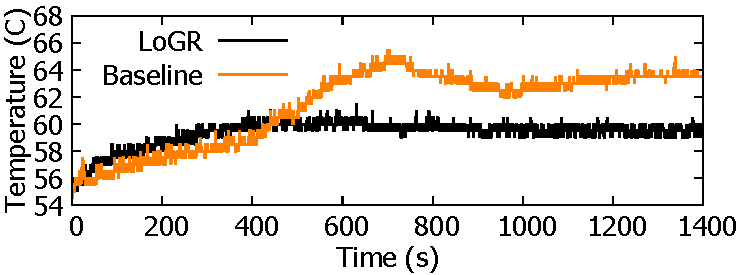
\includegraphics[width=0.46\linewidth]{frame_rate_heat-h_cropped}
        \label{fig:magicleap-heat}
    }
    \subfigure[Magic Leap One frame rate]{
        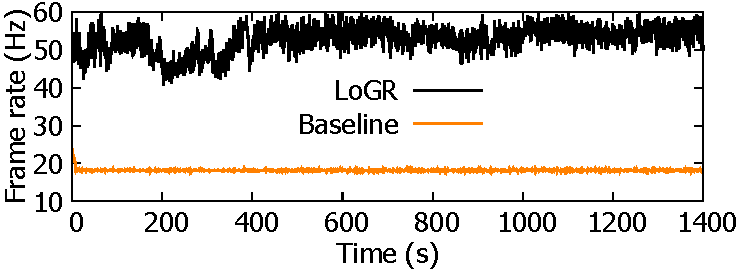
\includegraphics[width=0.46\linewidth]{frame_rate_heat-fr_cropped}
        \label{fig:magicleap-framerate}
    }
    \subfigure[Hololens device heating]{
        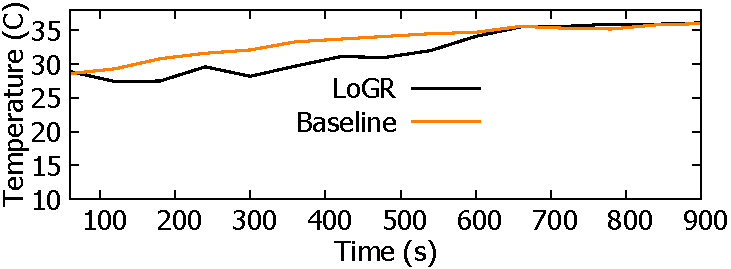
\includegraphics[width=0.46\linewidth]{hololens_heat_cropped}
        \label{fig:hololens-heat}
    }
    \subfigure[Hololens frame rate]{
        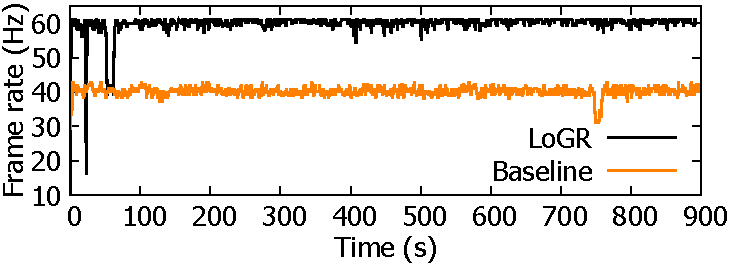
\includegraphics[width=0.46\linewidth]{hololens_frame_rate_cropped}
        \label{fig:hololens-framerate}
    }
    \vspace{-2ex}
    \caption{Temperature and achieved frame rate for the {\mlo} and Microsoft Hololens}
    \label{fig:temp-all}
\end{figure}


%\begin{figure}[t]
%    \centering
%    \vspace{-1ex}
%    \subfigure[Device temperature]{
%       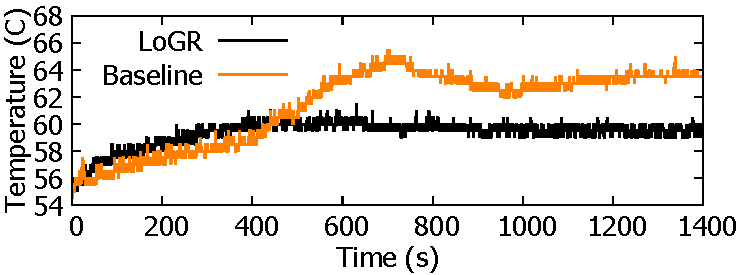
\includegraphics[width=0.46\linewidth]{frame_rate_heat-h_cropped}
%        \label{fig:magicleap-heat}
%    }
%    \subfigure[Achieved frame rate]{
%        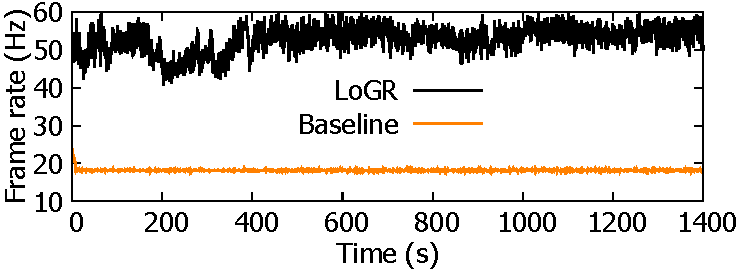
\includegraphics[width=0.46\linewidth]{frame_rate_heat-fr_cropped}
%        \label{fig:magicleap-framerate}
%    }
%    \vspace{-2ex}
%    \caption{Temperature and achieved frame rate for the {\mlo}. \jk{change to baseline}}
%    \label{fig:magicleap-all}
%\end{figure}

%\begin{figure}[t]
%    \centering
%    \vspace{-1ex}
%    \subfigure[Device temperature]{
%       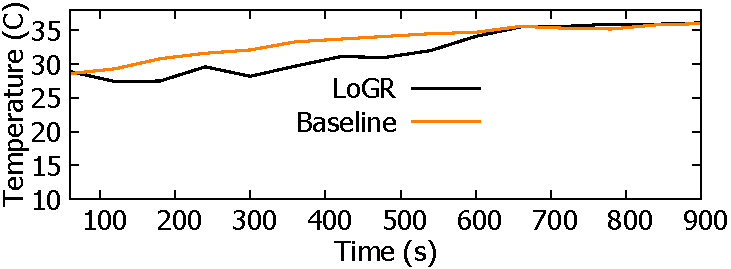
\includegraphics[width=0.46\linewidth]{hololens_heat_cropped}
%        \label{fig:hololens-heat}
%    }
%    \subfigure[Achieved frame rate]{
%        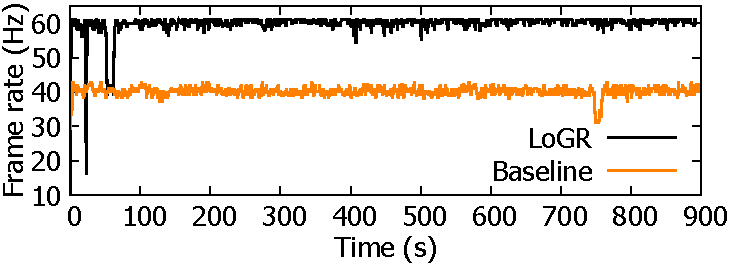
\includegraphics[width=0.46\linewidth]{hololens_frame_rate_cropped}
%        \label{fig:hololens-framerate}
%    }
%    \vspace{-2ex}
%    \caption{Temperature and achieved frame rate for the Microsoft Hololens. \jk{change to baseline}}
%    \label{fig:hololens-all}
%\end{figure}


Finally, we also see device heating as another important factor to consider as mobile AR headsets are worn directly on the head, and high operation temperatures can negatively affect the usability. Therefore, we measure the temperature of the {\mlo} and the Microsoft Hololens with and without applying {\myit} using a dynamic application that saturates the GPU's performance. Specifically, we record how the GPU/device temperature changes over time, along with their achieved frame rates and present the results in \fig\ref{fig:temp-all} for {\mlo} and Hololens. Note that the {\mlo}'s processing units are external to the headset. The users can carry an external processing unit wired to the headset device. On the other hand, on the Hololens, all processing units are integrated to the forehead component of the headset itself. Measuring heat on the {\mlo} was done using its power and thermal profiler and we present the GPU temperature, which dominates the processing unit's temperature. As the Hololens does not provide such analysis software, we used an infrared thermal camera to capture its forehead processing unit temperature on a per-minute basis.


From \fig\ref{fig:magicleap-heat}, we observe that, on the {\mlo}, the GPU temperature of the baseline saturates at a higher level compared to {\myit} and that {\myit}'s achieved frame rate is consistently higher. We see similar patterns for the Hololens (\figs\ref{fig:hololens-heat} and~\ref{fig:hololens-framerate}). 

%Note: the GPU saturates as a similar temperature but achieve a higher frame rate %in general.

%Note: the {\mlo}'s external GPU saturates as a similar temperature as the Hololens but achieve a higher frame rate in general.

%that the device temperature for the two schemes saturate as a similar level, but %differences in frame rates suggest that {\myit} offers higher quality contents %with same amount of heat generation. 


%achieves a high frame rate to tolerate the amount of scene dynamics, the baseline %scheme cannot accommodate for the such dynamics and the frame rate drops to $<$20. 
%
%We conducted this experiment with two device such as magic leap one that we deal with this study mainly and additional hololens. 
%
%

%As shown in the \fig\ref{fig:magicleap-heat}, the temperature of the magic leap one was higher at first when {\myit} was applied, but it did not rise above a certain temperature and maintained at about 60 ° C. When {\myit} was not applied, it rose to 65.5 ° C and maintained at about 63.5 degrees. At this time, in \fig\ref{fig:magicleap-framerate}, the frame rete when {\myit} is applied is going up and down between 50-60, but when it is not applied, it is kept at a little lower than 20. 
%
%This is because the HMD itself artificially lowers the frame rate in order to reduce the heating value. 
%
%In the case of hololens, it is seen that {\myit} is lower than when the heat rise rate is not applied, and the frame rate is also close to 60 when {\myit} is applied similar to magic leap one, but {\myit} is applied If you do not, you can see that it is kept at around 40. As can be seen from the two devices, the application of {\myit} shows that it can maintain a high frame rate while reducing the calorific value.
